\documentclass[oneside,14pt]{extarticle}
\usepackage{cmap}
\usepackage[utf8]{inputenc}
\usepackage[english,ukrainian]{babel}
\usepackage{graphicx}
\usepackage{geometry}
\usepackage{listings}
\usepackage{float}
\usepackage{amsmath}
\usepackage{subfig}
\usepackage{enumitem}
\geometry{
	a4paper,
	left=20mm,
	right=20mm,
	top=15mm,
	bottom=15mm,
}
\lstset{
	language=c,
	tabsize=4,
	keepspaces,
	showstringspaces=false,
	frame=single,
	language=python,
	breaklines=true,
	postbreak=\mbox{{$\hookrightarrow$}\space},
}
\graphicspath{ {./pictures} }
\setlength{\parindent}{4em}

\newcommand\subject{Основи програмування вбудованих систем}
\newcommand\lecturer{професор кафедри ПЗ\\Гавриш В.І.}
\newcommand\teacher{доцент кафедри ПЗ\\Крук О.Г.}
\newcommand\mygroup{ПЗ-32}
\newcommand\lab{2}
\newcommand\theme{Моделювання дискретних $2\pi$- періодичних сигналів квадратичним
поліномом та рядом Фур’є (перший спосіб)}
\newcommand\purpose{Поданий у дискретному вигляді $2\pi$- періодичний сигнал
наблизити рядом Фур’є та апроксимувати поліномом другого степеня,
коефіцієнти якого визначити за методом найменших квадратів. Виконати
геометричне зображення сигналу, його апроксимації квадратичним поліномом
та наближення рядом Фур’є. Визначити середню абсолютну похибку
апроксимації та наближення}

\begin{document}
\begin{normalsize}
	\begin{titlepage}
		\thispagestyle{empty}
		\begin{center}
			\textbf{МІНІСТЕРСТВО ОСВІТИ І НАУКИ УКРАЇНИ\\
				НАЦІОНАЛЬНИЙ УНІВЕРСИТЕТ "ЛЬВІВСЬКА ПОЛІТЕХНІКА"}
		\end{center}
		\begin{flushright}
			\textbf{ІКНІ}\\
			Кафедра \textbf{ПЗ}
		\end{flushright}
		\vspace{120pt}
		\begin{center}
			\textbf{ЗВІТ}\\
			\vspace{10pt}
			до лабораторної роботи № \lab\\
			\textbf{на тему}: <<\textit{\theme}>>\\
			\textbf{з дисципліни}: <<\subject>>
		\end{center}
		\vspace{40pt}
		\begin{flushright}
			
			\textbf{Лектор}:\\
			\lecturer\\
			\vspace{28pt}
			\textbf{Виконав}:\\
			
			студент групи \mygroup\\
			Коваленко Д.М.\\
			\vspace{28pt}
			\textbf{Прийняв}:\\
			
			\teacher\\
			
			\vspace{28pt}
			«\rule{1cm}{0.15mm}» \rule{1.5cm}{0.15mm} 2024 р.\\
			$\sum$ = \rule{1cm}{0.15mm}……………\\
			
		\end{flushright}
		\vspace{\fill}
		\begin{center}
			\textbf{Львів — 2024}
		\end{center}
	\end{titlepage}
		
	\begin{description}
		\item[Тема.] \theme.
		\item[Мета.] \purpose.
	\end{description}

	\section*{Індивідуальне завдання}
	\begin{enumerate}
		\item Поданий у дискретному вигляді $2\pi$- періодичний сигнал апроксимувати
поліномом другого степеня, коефіцієнти якого визначити за методом найменших
квадратів.
		\item Дискретно поданий $2\pi$- періодичний сигнал наблизити рядом Фур’є.
		\item Виконати геометричне зображення дискретного сигналу та кривих, які
описано апроксимаційним квадратичним поліном і рядом Фур’є;
		\item Визначити середні абсолютні похибки, отримані за наближенням
квадратичного полінома та ряду Фур’є.
	\end{enumerate}
	
	\subsection*{Варіант №6}
	
	\begin{equation}
		4,44; 5,43; 6,01; 7,35; 8,07; 9,89\nonumber
	\end{equation}
	
	\section*{Хід роботи}	

	\subsection*{Код програми}
	Файл \textit{main.py}:
	{\small
		\begin{lstlisting}
import numpy as np
import matplotlib.pyplot as plt

y = np.array([4.44, 5.43, 6.01, 7.35, 8.07, 9.89])
n = len(y)
x = np.linspace(-np.pi, np.pi, n)

def polynomial_approximation(x, y):
    coeffs = np.polyfit(x, y, 2)
    y_poly = np.polyval(coeffs, x)
    mae_poly = np.mean(np.abs(y - y_poly))
    rmse_poly = np.sqrt(np.mean((y - y_poly)**2))
    return y_poly, mae_poly, rmse_poly, coeffs

def fourier_series(x, y):
    a_0 = np.sum(y) * 2 / n
    a_k = lambda k: np.sum(y * np.cos(k * x)) * 2 / n
    b_k = lambda k: np.sum(y * np.sin(k * x)) * 2 / n
    
    return lambda x: a_0 / 2 + sum(a_k(k) * np.cos(k * x) + b_k(k) * np.sin(k * x) for k in range(1, 5))

y_poly, mae_poly, rmse_poly, coeffs_poly = polynomial_approximation(x, y)
fourier_func = fourier_series(x, y)
y_fourier = fourier_func(x)
mae_fourier = np.mean(np.abs(y - y_fourier))
rmse_fourier = np.sqrt(np.mean((y - y_fourier)**2))

plt.figure(figsize=(10, 6))
plt.plot(x, y, 'o', label='Original Signal')
plt.plot(x, y_poly, '-', label='Quadratic Polynomial Approximation')
plt.plot(x, y_fourier, '--', label='Fourier Series Approximation', linewidth=2)
plt.legend()
plt.xlabel('x')
plt.ylabel('y')
plt.title('Signal Approximation')
plt.show()

print(f"MAE for Quadratic Polynomial: {mae_poly}")
print(f"RMSE for Quadratic Polynomial: {rmse_poly}")
print(f"MAE for Fourier Series: {mae_fourier}")
print(f"RMSE for Fourier Series: {rmse_fourier}")
print(f"Coefficients: {coeffs_poly}")\end{lstlisting}
	}
	
	\subsection*{Виконання програми}
	
	\begin{figure}[H]
		\centering
		\vspace{-30pt}
		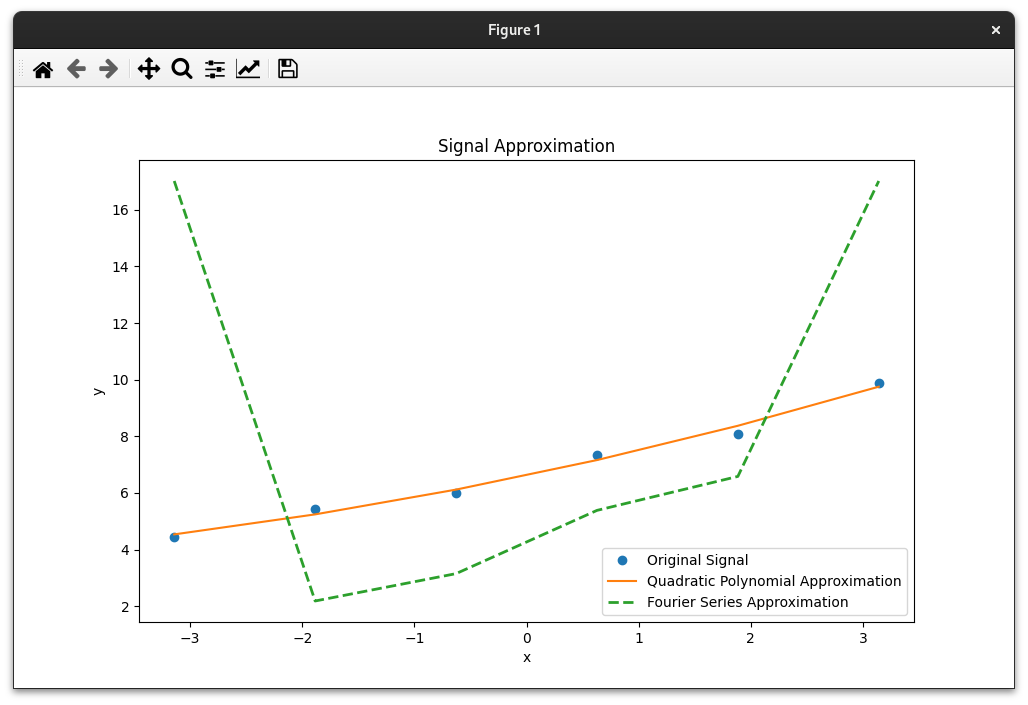
\includegraphics[scale=0.48]{1}
		\vspace{-30pt}
		\caption{Геометричне зображення апроксимації дискретного сигналу апроксимаційним
поліномом та рядом Фур’є.}
	\end{figure}
	
	\begin{table}[H]
		\centering
		\renewcommand{\arraystretch}{1.5}
		\begin{tabular}{|c|c@{\hspace{15pt}}|c@{\hspace{15pt}}|}
			\hline
			Метод & Сер. абс. похибка & Сер. квад. похибка\\ \hline
			Фур'є & 4.87 & 6.24 \\ \hline
			Кв. Поліном & 0.17 & 0.18 \\ \hline
		\end{tabular}
		\caption{Порівняння середньої абсолютної похибки та середньої квадратичної похибки.}
	\end{table}
	
	\section*{Висновки}
	Під час виконання лабораторної роботи я наблизив рядом Фур’є та апроксимував поліномом другого степеня поданий у дискретному вигляді $2\pi$- періодичний сигнал,
коефіцієнти якого визначив за методом найменших квадратів. Виконав
геометричне зображення сигналу, його апроксимації квадратичним поліномом
та наблизив рядом Фур’є. Визначив середню абсолютну похибку
апроксимації та наближення.
	    
\end{normalsize}
\end{document}
